\section{Software architecture}

In this section the software for the simulator is described. The
program is following the concept of the MIPS architecture, using
classes for components.

\begin{figure}[h]
    \centering
    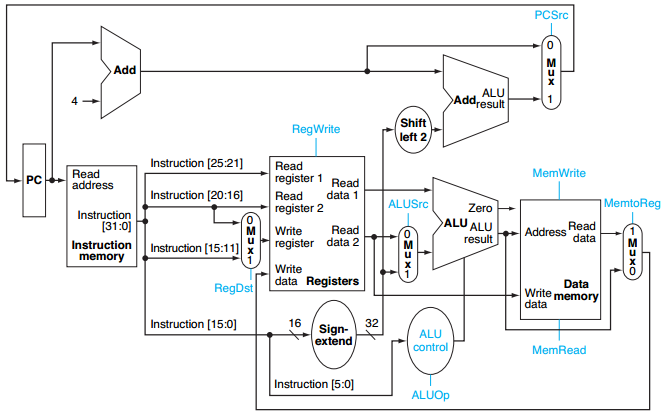
\includegraphics[scale=0.6]{images/datapath-r-format}
    \caption{MIPS representation\cite{Patterson:2008:COD:1502247} of the data path on R-formatted Instruction}
    \label{fig:datapathBranchOnEqual}
\end{figure}

\subsection{Simulator}
The class \texttt{Simulator} control the signals between the different components.

When an Instruction is fetched and executed, the method
\texttt{execute} is called. The following flow can be described for an
\emph{R-format} Instruction with op-code 0:


\begin{enumerate}
\item The PC will be incremented (current + 4).
\item ALU Controller will be called with the OpCode (True values:\emph{regDst, regWrite, aluOp1}).
\item Requested read-register from the Instruction is fetched from the \texttt{Register memory} is be called.
\item The fetched registers value will be sent to the ALU.
\item The output of the ALU will be saved in a register.
\end{enumerate}

The \texttt{Simulator} is the only class that can not be translated
into a component of the MIPS architecture but should be seen as the
signals that is sent between the components. It will also take care of
\texttt{MUX} conditions and the \texttt{Shift left 2} components.


\subsubsection{Component PC}

The component \texttt{Program Counter} is the class \texttt{PC}. The
class responsibility is to know what Instruction that will be read and
executed next. Each instruction size is 4 byte in the
\texttt{Instruction Memory} so a increment will be \emph{current value
  + 4}.

\subsubsection{Component Instruction Memory}

The class \texttt{InstructionMemory} consist of all Instruction given
to the simulator, the \texttt{PC} will point to an Instruction in the
memory. The number of Instruction that will be possible can be
initilized with any given size, if no size is given then it will
automatically be able to save 250 Instruction, consisting of 4 bytes
(32 bits) each, i.e. 1000 bytes.

\newpage

\subsubsection{Component ALU Controller}

The \texttt{ALU controller} is represented as the Java class
\texttt{Control}. The class state is declared in booleans which in the
MIPS architecture is called \emph{control signals} , the state is
altered by calling the method \texttt{updateOperationType}. The method
takes an parameter with the opcode that consist of six bits. The bits
will be checked towards a truth table where the state is
determined. Each state will affect the in the architecture.

\begin{table}[H]
\centering
\begin{tabular}{l|cccccc}
\hline
\bf{Opcode}    &\bf{[000000]}&\bf{[100011]} &\bf{[101011]}  &\bf{[000100]}  &\bf{[001000]}  &\bf{[001101]} \\\hline
   regDst      &   T         &   F          &   X           &   X           &   F           &   F    \\\hline
   aluSrc      &   F         &   T          &   T           &   F           &   T           &   T    \\\hline
   memtoReg    &   F         &   T          &   X           &   X           &   T           &   T    \\\hline
   regWrite    &   T         &   T          &   F           &   F           &   F           &   F    \\\hline
   memRead     &   F         &   T          &   F           &   F           &   F           &   F    \\\hline
   memWrite    &   F         &   F          &   T           &   F           &   F           &   F    \\\hline
   branch      &   F         &   F          &   F           &   T           &   F           &   F    \\\hline
   aluOp1      &   T         &   F          &   F           &   F           &   F           &   T    \\\hline
   aluOp0      &   F         &   F          &   F           &   T           &   F           &   F    \\\hline
\end{tabular}
\caption{State of the Control class is decided by the opCode received to the method \texttt{updateOperationType}}
\label{table:AluControlState}
\end{table}

As seen in Table \ref{table:AluControlState} the truth table can
affect each control signal differently. An R-format with the opCode
[000000] will make it possible for simulator to write to the register
by the control signal \emph{regDst} and \emph{regWrite}. Also will the
control signal \emph{aluOp1} change the behavior of the
\texttt{ALUOperation}, seen in section \ref{sec:ALuOperation}.Since
the state of the class is controlling the \emph{control signals} the
communication will go between \texttt{Controller} and
\texttt{Simulator}

\subsubsection{Component ALU Operation}
\label{sec:ALuOperation}

The \texttt{ALU} named \texttt{ALUOperation} makes the arithmetic
operations from given registers and, if needed, store or load from the
\texttt{Data Memory}. Given the indata to the ALU, it will preform
different operations.

\begin{table}[H]
\centering
\begin{tabular}{ccc|l}
AluOp1&AluOp2   &funct      &Operation  \\\hline
1     & 0     & \texttt{100111}     &NOR         \\\hline
1     & 0     & \texttt{000010}     &SRL         \\\hline
1     & 0     & \texttt{000011}     &SRA         \\\hline
1     & X     & \texttt{XX0010}     &SUBTRACT    \\\hline
1     & 0     & \texttt{XX0000}     &ADD         \\\hline
1     & 0     & \texttt{XX0100}     &AND         \\\hline
1     & 0     & \texttt{XX0101}     &OR          \\\hline
1     & X     & \texttt{XX1010}     &SLT         \\\hline
0     & 0     & \texttt{XXXXXX}     &ADD         \\\hline
0     & 1     & \texttt{XXXXXX}     &SUBTRACT    \\\hline
1     & 0     & \texttt{XXXXXX}     &OR          \\\hline
\end{tabular}
\caption{ALU operation depending on what AluOp set in \texttt{Controller} and funct-field.}
\label{tab:ALUoperation}
\end{table}

As shown in table \ref{tab:ALUoperation} depending on the
\texttt{AluOp1} and \texttt{AluOp2} that are set in the
\texttt{Controller} but also the funct-field in the Instruction.

\subsubsection{Component SignExtender}

The component as well as the class \texttt{SignExtender} will take a
given value and extend it. For the purpose in MIPS it will take a 16
bits value and transform it to a 32 bit. This is used on \texttt{jump}
and \texttt{branch} Instructions.

\subsubsection{Component Data Memory}

The \texttt{DataMemory} class concist of 1000 \texttt{ByteBuffer}s to
simulate the Data memory in the MIPS architecture.
